\chapter{Evaluation}\label{ch:evaluation}
Parameters of models
\section{Similarity measurements}\label{sec:evaluation-sim-measurements}

According to \citeauthor{HfsentTrans2019}, the similarity measurements discussed above obtained roughly the same results in their experiments \cite{HfsentTrans2019}.   


\subsection{\eigendocs{}}\label{subsec:evaluation-eigendocs}
% number of components
In order to determine the optimal number of components used for \eigendocs{} the cumulative explained variance and the reconstruction error were plotted 
as displayed in \autoref{fig:det_n_comp} from \autoref{subsec:eigenface}.
The first plot indicated that 90\% of the variance is explained by 95 components.
Usually, that would have been the number of dimensions of the subspace onto which the documents would have been projected.
However, when working with cluster algorithms like \ac{optics} prior to this step, the number of dimensions should be reduced even further to achieve valid clusters.
Therefore the second approach was used.
The second plot showed the reconstruction error with respect to different numbers of components.
\textcolor{red}{"knees"} were visible at 10 and 13.
Since visual inspection accounted for the fact that the decline of the reconstruction error after 13 declined more than after 10, the number of components chosen is 13.

% results
The results of the \eigendocs{} algorithm are displayed in \autoref{fig:preprocessed_docs_eigendocs}.

\begin{figure}[htp] % htp = hier (h), top (t), oder auf einer eigenen Seite (p).
    \centering
    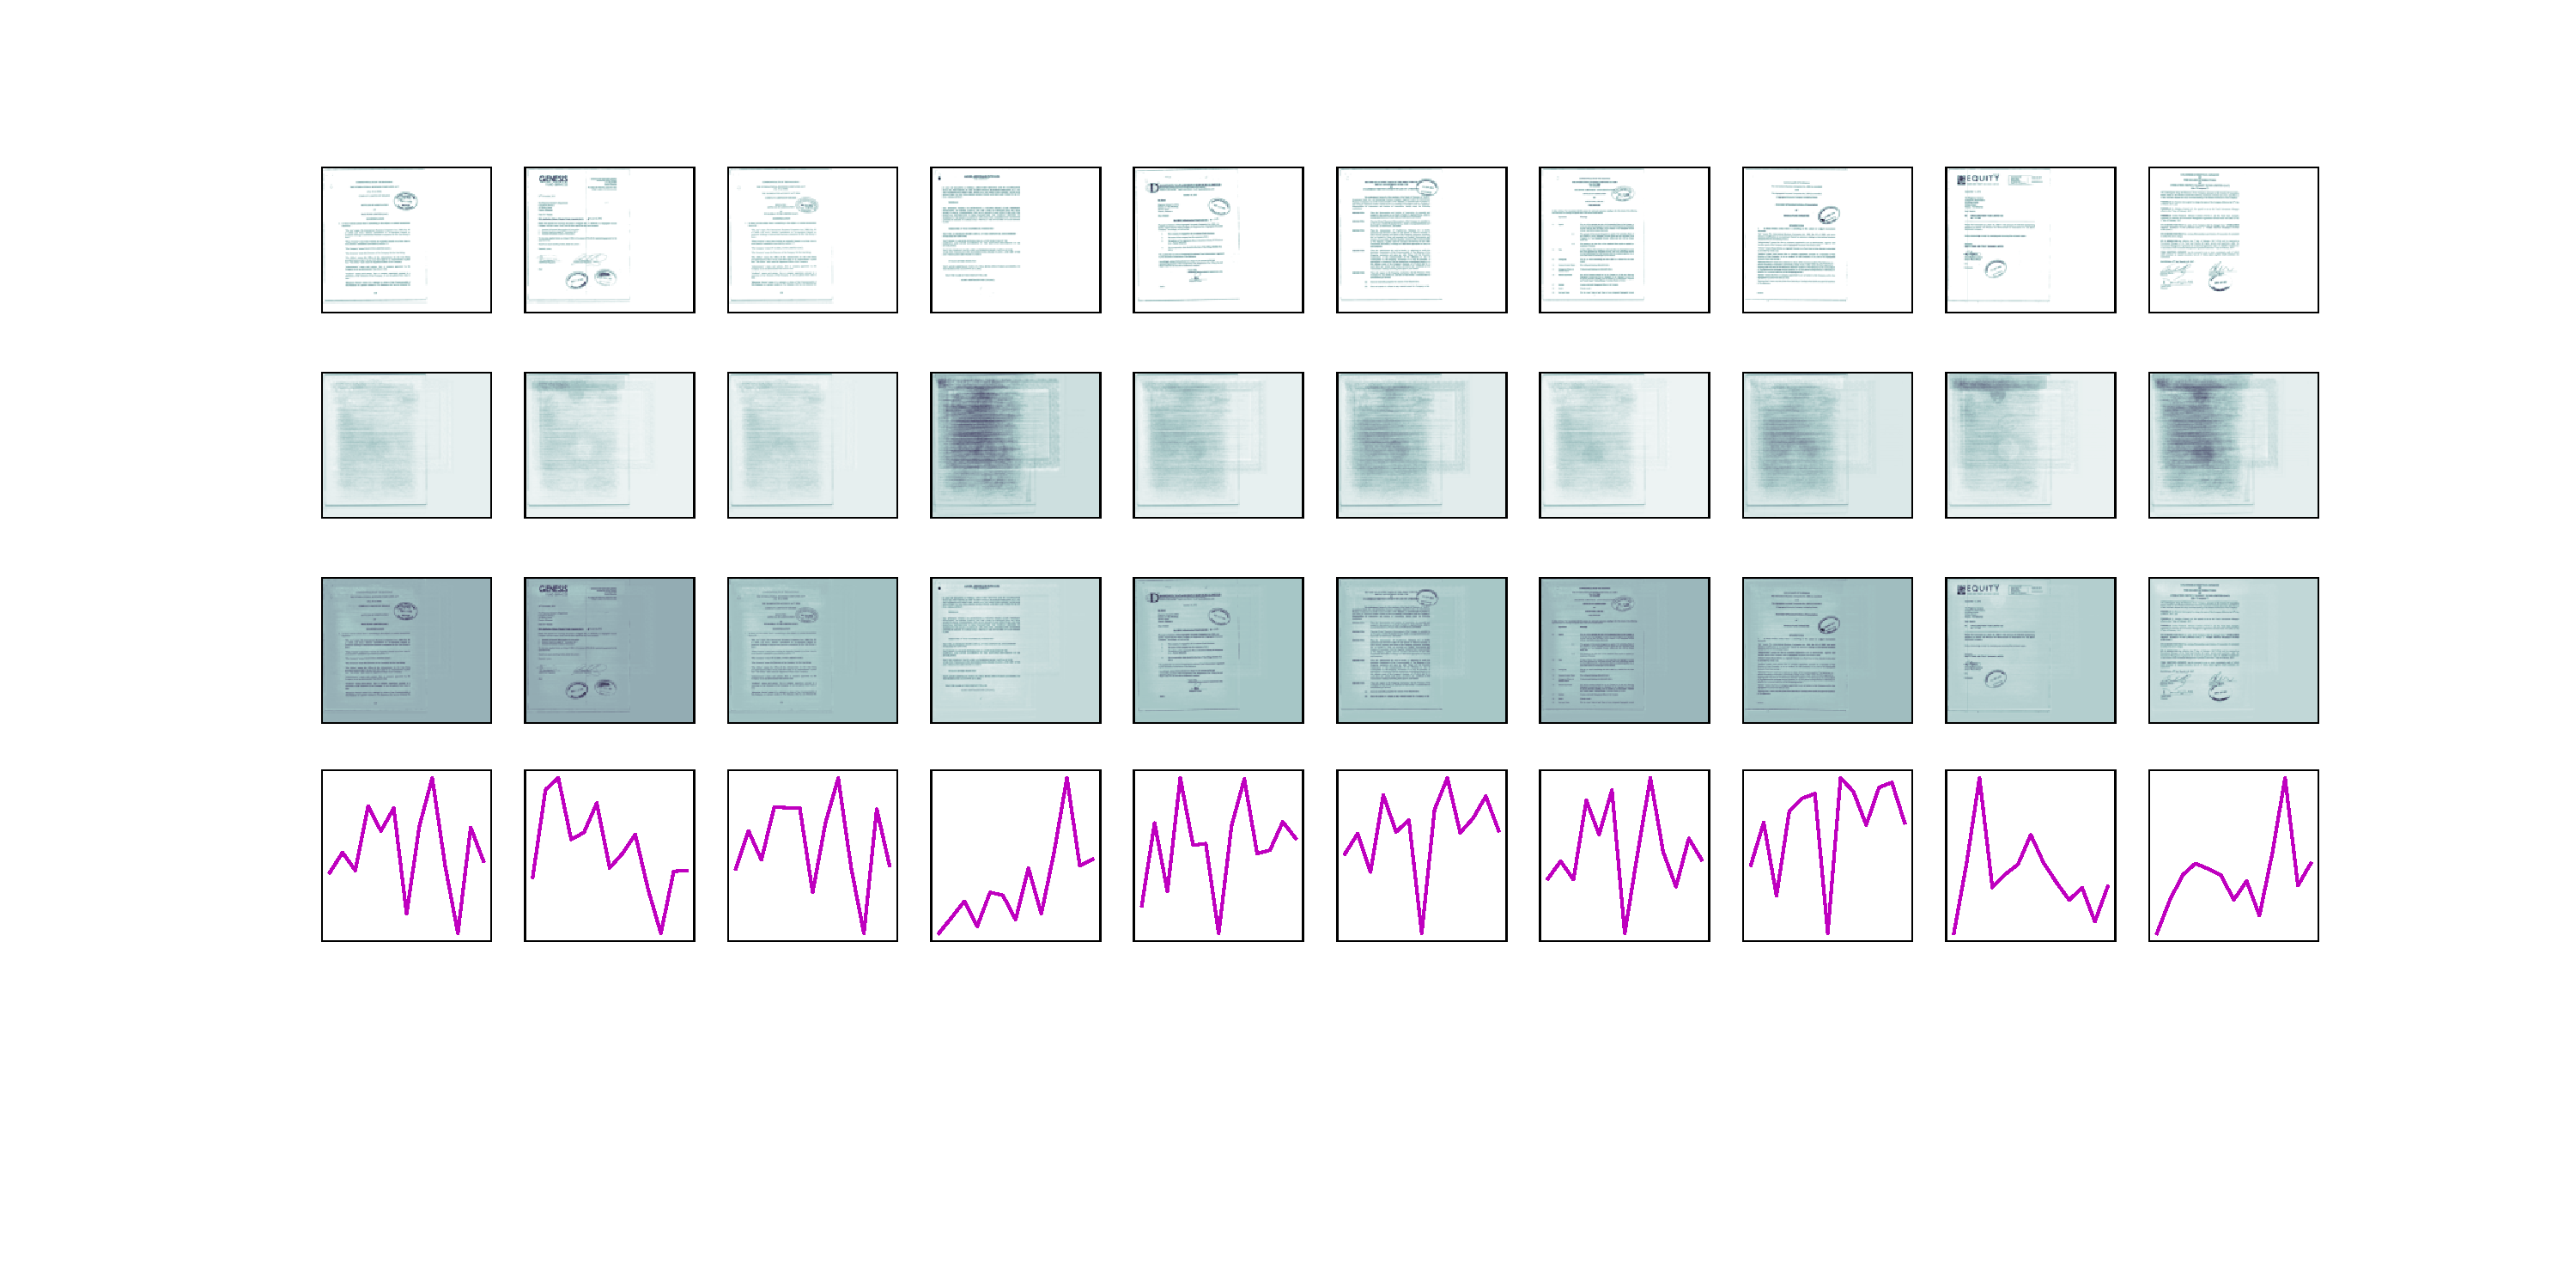
\includegraphics[width=0.7\textwidth]{images/Eigendocs/transformation/eigendocs_13dims.pdf}
    \caption{The first 10 preprocessed documents of the dataset.
    The original images are displayed in the first row.
    The second row shows the reconstructed images using the compressed images from the fourth row.
    The third row shows the reconstruction error, i.e. the difference between the reconstructed and the original image.
    The last row presents the greyscale values of the compressed 13-dimensional image as a line.
    }
    \label{fig:preprocessed_docs_eigendocs}
\end{figure}

\section{Evaluation of \ac{ae}}\label{sec:evaluation-ae}

% architecture
In order to determine, which architecture for the latent/ hidden space of the \ac{ae} is the best option, 
different architectures were tested and compared in terms of \ac{rsme} and cosine similarity.
The \ac{rsme} is calculated as given in \lst{lst:impl-rsme}.
The cosine similarity is calculated as given in \lst{lst:impl-cos_sim}.
The dataset used for the evaluation is a selection of 195 documents from the Bahamas dataset.

% RSME
\begin{listing}[htp]
    \begin{minted}{python3}
        rsme = np.linalg.norm(inverse_embedding - embeddings) 
                / np.sqrt(embeddings.shape[0])
    \end{minted}
    \caption{
        Computation of the \ac{rsme} between the original and the reconstructed embedding.
    }
    \label{lst:impl-rsme}
\end{listing}

% cosine similarity
\begin{listing}[htp]
    \begin{minted}{python3}
        cos_sim = statistics.mean([np.dot(inverse_emb, embedding)
                /(np.linalg.norm(inverse_emb)*np.linalg.norm(embedding)) 
                for inverse_emb, embedding in zip(inverse_embedding, embeddings)])
    \end{minted}
    \caption{
        Computation of the cosine similarity between the original and the reconstructed embedding.
    }
    \label{lst:impl-cos_sim}
\end{listing}

The scores of different architectures are shown in \fig{fig:eval-ae-architecture}.
While most of the architectures produced similar results, one architecture stood out.
Combining 2500, 3000 and 3500 dimensions in the hidden space produced the worst \ac{rsme} results.
The best results were achieved by adding 3500-dimensional layers in the hidden space.
However, the results of the best architecture do not differ greatly from the others.

\begin{figure}[h] % htp = hier (h), top (t), oder auf einer eigenen Seite (p).
    \centering
    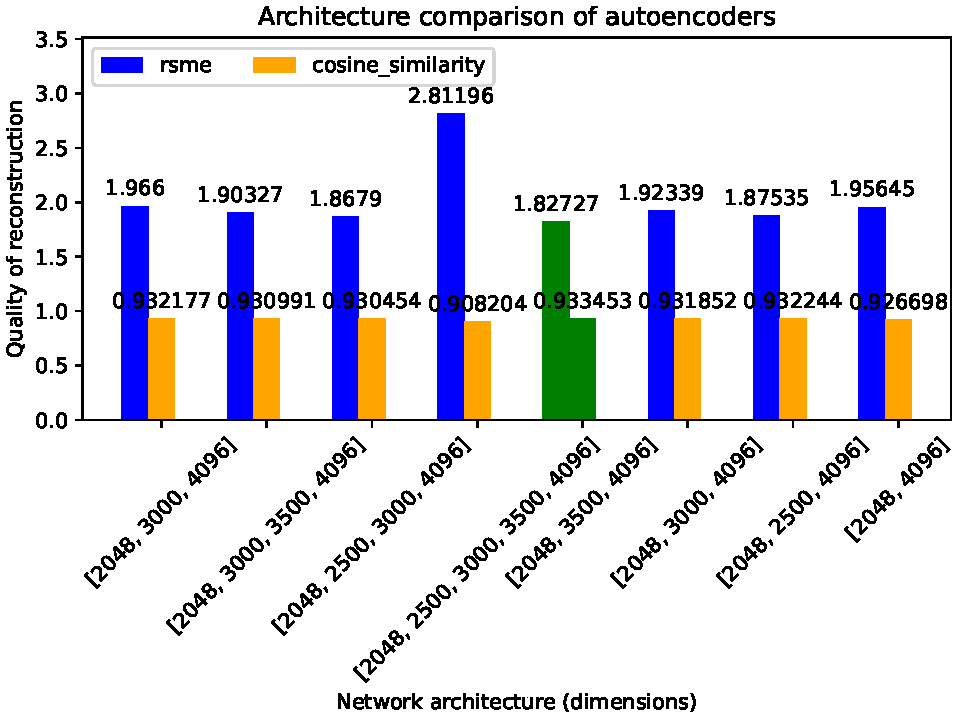
\includegraphics[width=0.7\textwidth]{images/embeddings/autoencoder/ae_score_plot.pdf}
    \caption{The effect of different \ac{ae} architectures on the reconstruction error.
    The error is measured in terms of \ac{rsme} (blue bars) and cosine similarity (yellow bars) between the original and the reconstructed image.
    The smallest \ac{rsme} and the biggest cosine similarity belong to the architecture best suitable to this task and are coloured green.
    }
    \label{fig:eval-ae-architecture}
\end{figure}

\subsection{Evaluation of \ac{optics}}\label{subsec:evaluation-OPTICS}

\textcolor{red}{TODO: compare preprocessing results}


% preprocessed images
\begin{figure}[htp] % htp = hier (h), top (t), oder auf einer eigenen Seite (p).
    \centering
    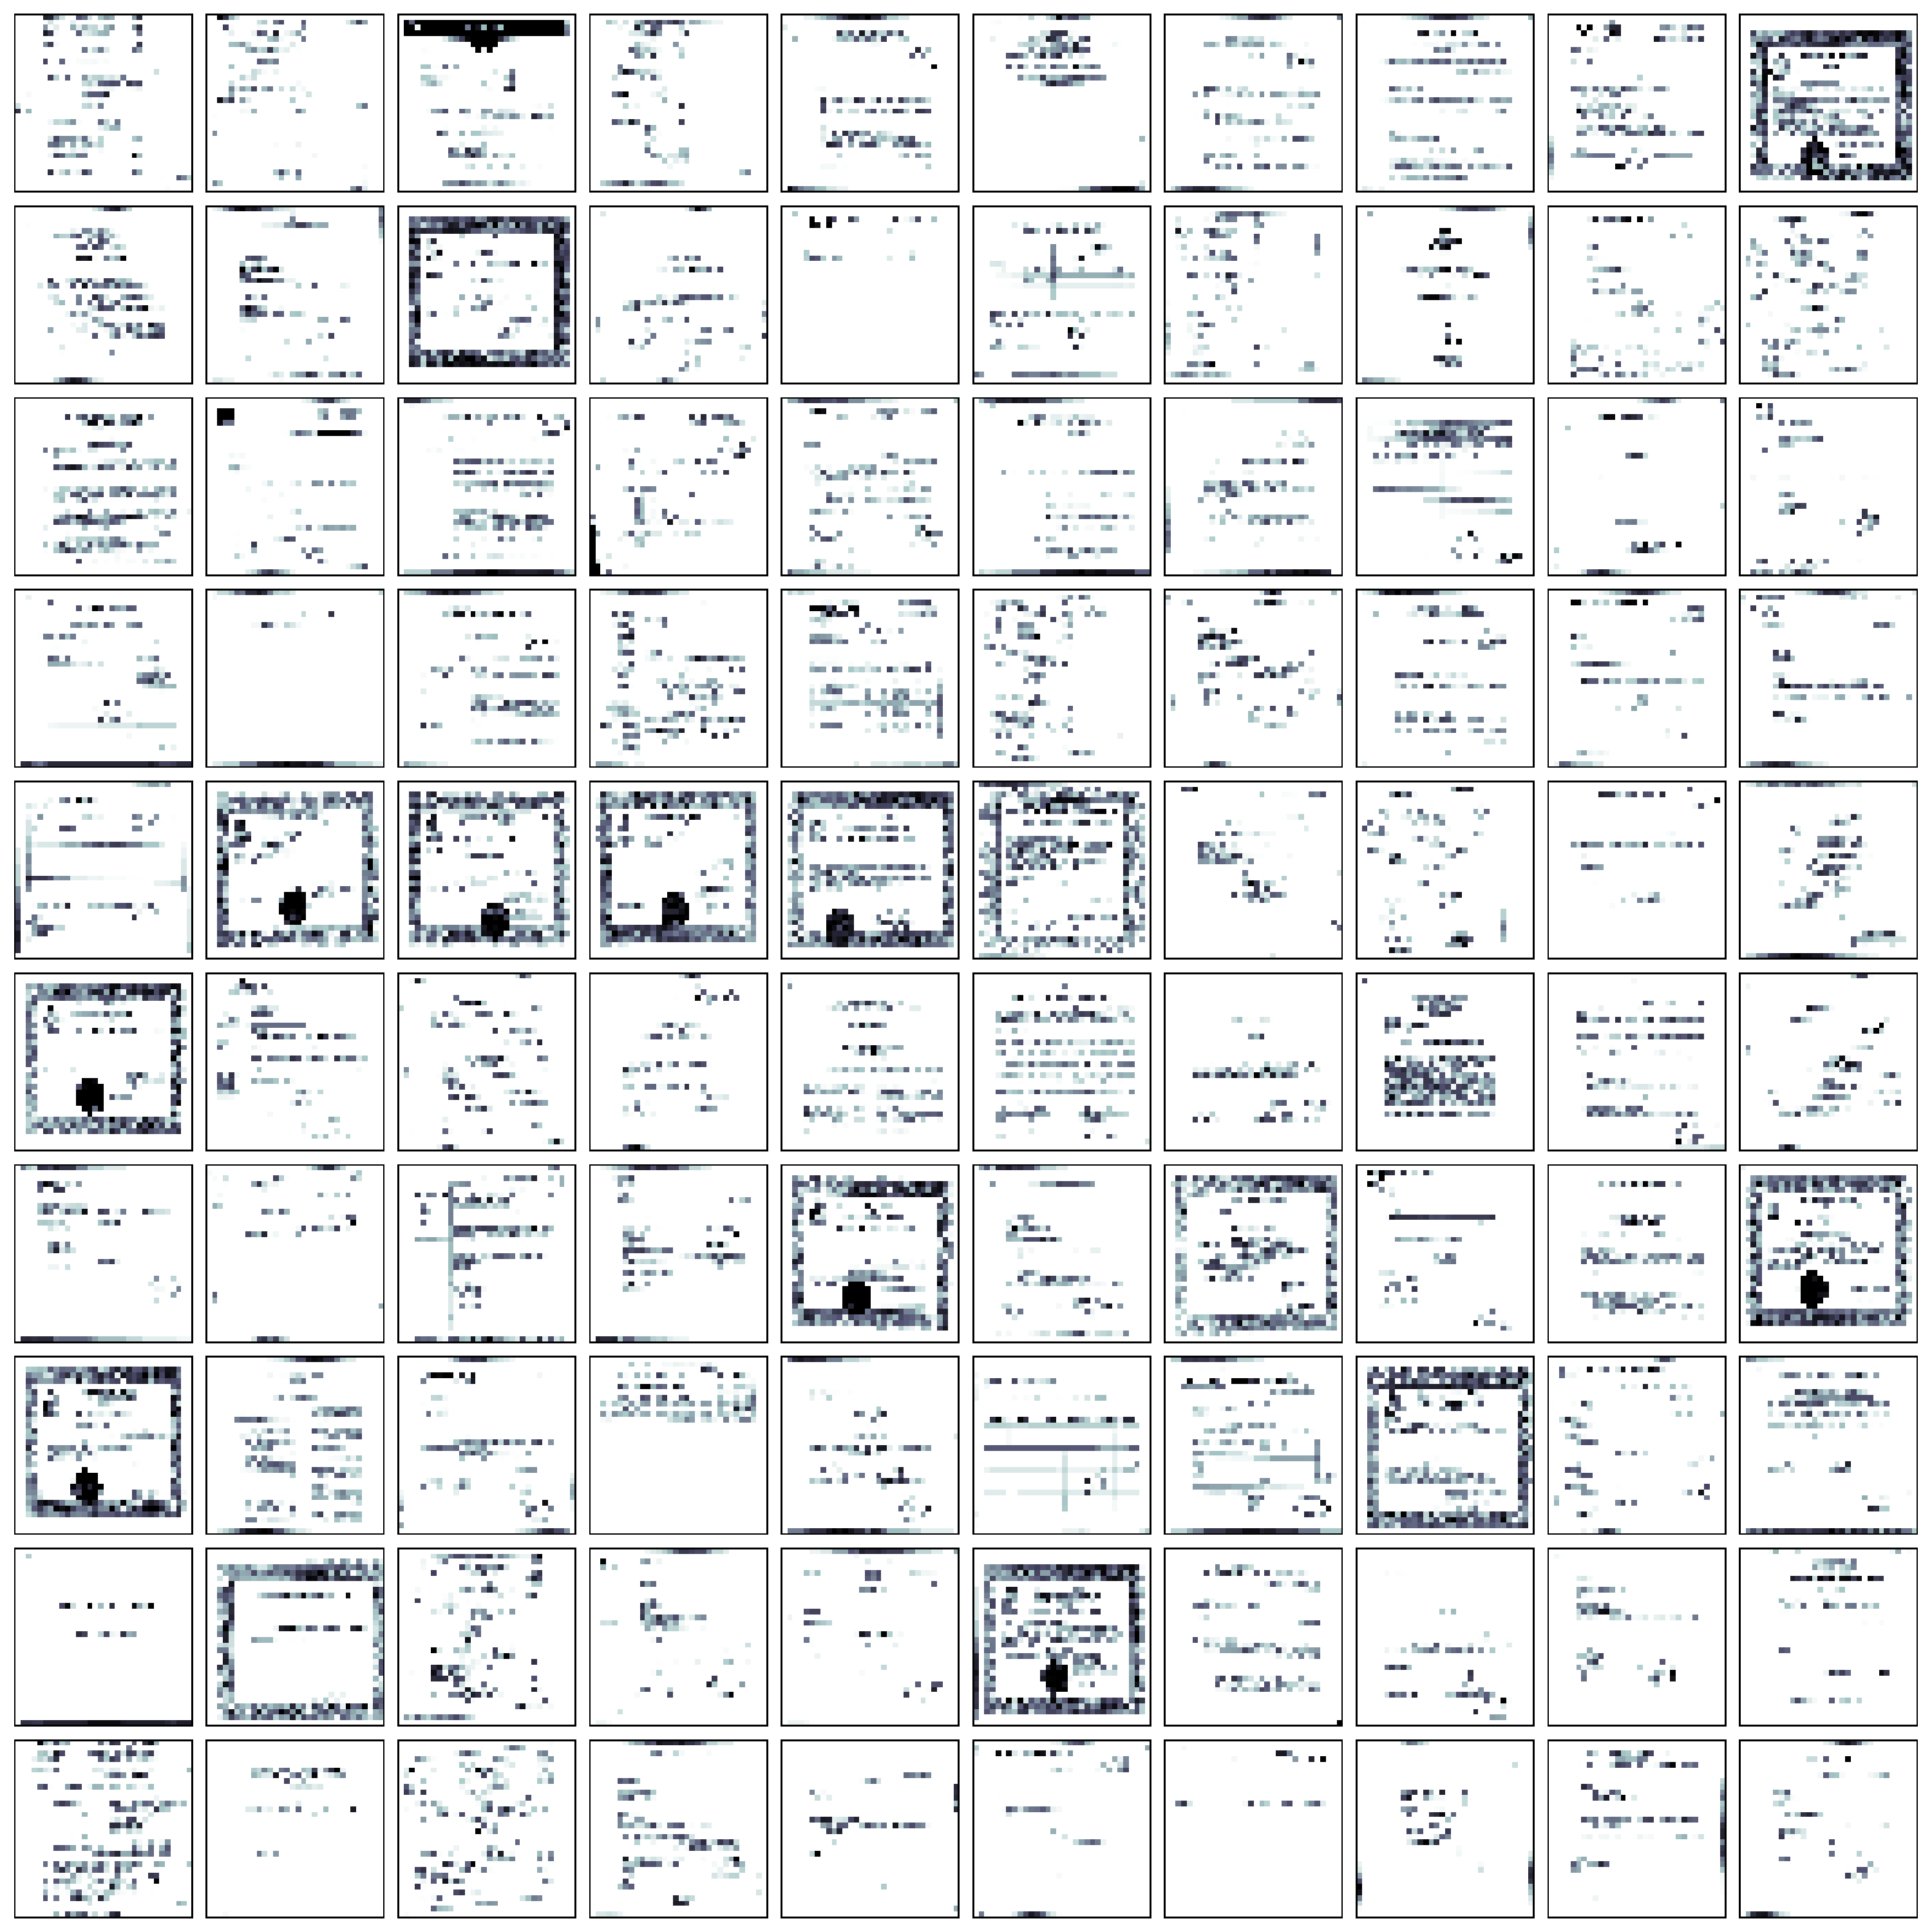
\includegraphics[width=0.5\textwidth]{images/OPTICS/32x32/preprocessed_docs.pdf}
    \caption{The first 100 preprocessed documents of the dataset.
    They were preprocessed in order to have the same characteristics as the images used in \cite{OPTICS1999}.
    The images were preprocessed as discussed in \autoref{pt:32} to 32x32 greyscale pixels, which drastically reduced the quality of the images.
    }
    \label{fig:preprocessed_docs_32x32}
\end{figure}




% OPTIC cluster results
\begin{figure}%
    \centering
    \subfloat[\centering The clusters identified by \ac{optics} of the documents preprocessed according to \autoref{pt:32}.]{{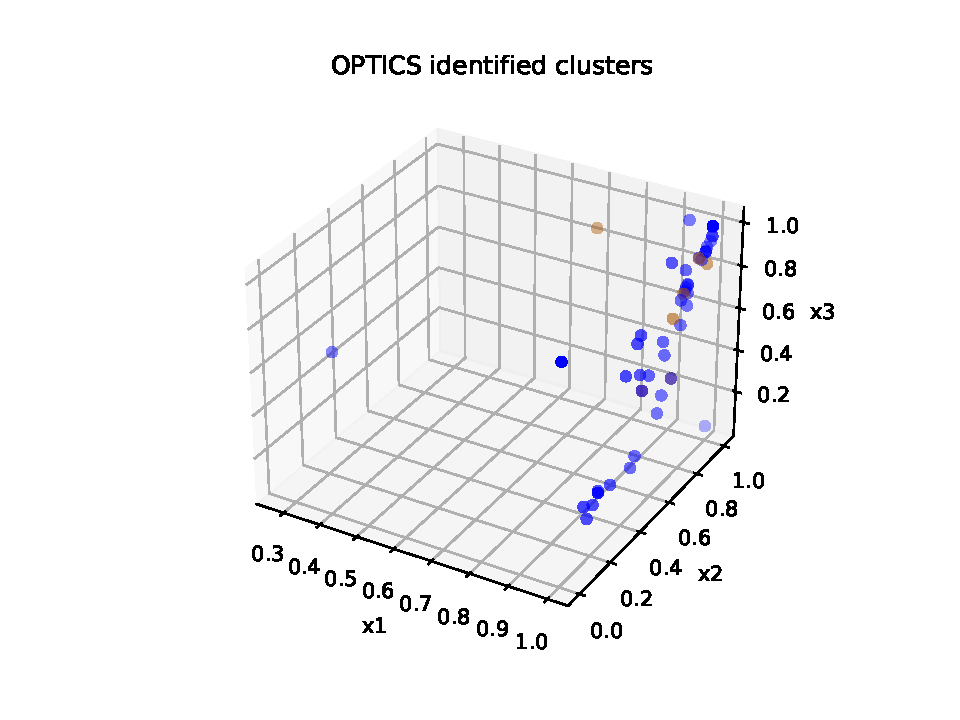
\includegraphics[width=5cm]{images/OPTICS/32x32/OPTICS_cluster_32x32.pdf} }}%
    \qquad
    \subfloat[\centering The clusters identified by \ac{optics} of the documents preprocessed according to \autoref{pt:eigendocs}.]{{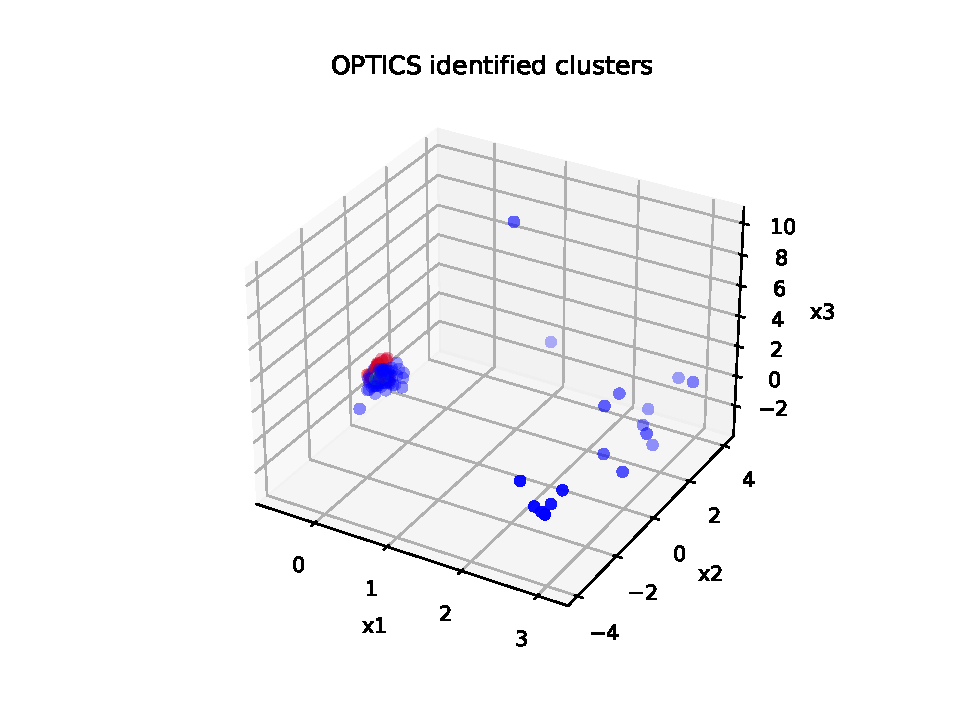
\includegraphics[width=5cm]{images/OPTICS/eigendocs/OPTICS_cluster_eigendocs.pdf} }}%
    \caption{The clusters were extracted from the respective reachability plot in \autoref{fig:reachability_plots}.
    The blue points are noise points, whereas any other colour denotes a cluster.}%
    \label{fig:optics_cluster}%
\end{figure}

\section{Evaluation of database}\label{subsec:evaluation-db}

According to \cite{flask_book2018}, \ac{sql} databases are a good choice for efficiently storing structured data.
This is because their paradigm \acs{acid}, i.e. \acl{acid}, provides high reliability.
\ac{nosql} databases, on the other hand, are more flexible and can be used to store unstructured data \cite{flask_book2018}.
They do not require a predefined schema and can therefore accept documents of arbitrary structure \cite{flask2018}.

Usually, \ac{nosql} databases do not offer services such as \texttt{JOIN} \cite{flask2018}.
According to \citeauthor{flask2018}, \ac{nosql} databases make a tradeoff between storage and speed, as well as a tradeoff between consistency and availability.
\ac{nosql} databases are said to outperform out-of-the-box \ac{sql} databases \cite{flask2018}.

A document store database can be used if the primary goal is to write fast rather than write save \cite{flask2018}.

\section{Evaluation of \acs{tfidf}}\label{sec:evaluation-tfidf}

The main obstacle to overcome was the high dimensionality of the \ac{tfidf} embeddings.
Hence, the goal of the parameter selection was to find a way to reduce the dimensionality of the vocabulary to the maximum vector dimensionality of \databaseName{}.
However, the quality of the embeddings should not decline too much.

% parameter selection
The choice of the preprocessor was investigated with regard to the goal of minimizing the vocabulary size.
Both the default and custom preprocessor were tested on a data corpus of 195 documents with regard to the vocabulary (size) and the result of preprocessing.
While the default preprocessor had a vocabulary size of 1641, the custom preprocessor had a size of 1906.
The custom preprocessor was chosen because it had a smaller vocabulary size and TODO: vocab of custom.

% two fields in db
Initially, there should have been two different \ac{tfidf} models.
The first one should have been used to obtain documents which are similar to the query document.
Therefore, terms which occur only once in the corpus should have been removed from the vocabulary.
The second approach should have been used to obtain specific documents from the corpus.
Hence, the vocabulary should consist of very document-specific terms and thus, \texttt{max\_df} would have been relatively low, to omit terms that occur in many documents.
However, the restrictions imposed by the database implementation made it impossible to explore many parameter ranges.
Therefore, only one \ac{tfidf} model was used in the end, whose parameters \texttt{min\_df} and \texttt{max\_df} were set to values which kept the vocabulary and thus,
the dimensionality of the embeddings reasonably small.

\section{Evaluation of \ac{d2v}}\label{sec:evaluation-doc2vec}

Since no labelled data is available, the evaluation of the \ac{d2v} embeddings is limited.
Therefore, the \ac{d2v} embeddings are evaluated by comparing them to other embeddings.
The \ac{d2v} model is not tuned in terms of hyperparameter selection,
but the default settings are used since there is no way to evaluate the resulting embeddings.


\section{\infersent{}}\label{sec:evaluation-inferSent}

% pool type
The \texttt{max} pooling type is used for the \infersent{} model, since the \citeauthor{inferSent2018} 
found from conducting experiments using different pooling techniques
that it was the best option.

% version/ embeddings dictionary
Initially, in this work, the \ac{glove} word embeddings were used for the \infersent{} model.
However, since the file of precomputed \acs{glove} word embeddings has a size of 5.65 GB and thus,
slows down the model, ultimately another word embedding was used.
The time necessary to initialize the database, compute and insert 195 documents for specific embeddings is displayed in \autoref{fig:times_emb}.
The custom word embedding used in this work is a \ac{w2v} model trained on a selection of 195 documents from the Bahamas dataset.

\begin{figure}%
    \centering
    \subfloat[\centering Precomputed embeddings of \ac{glove}.]{{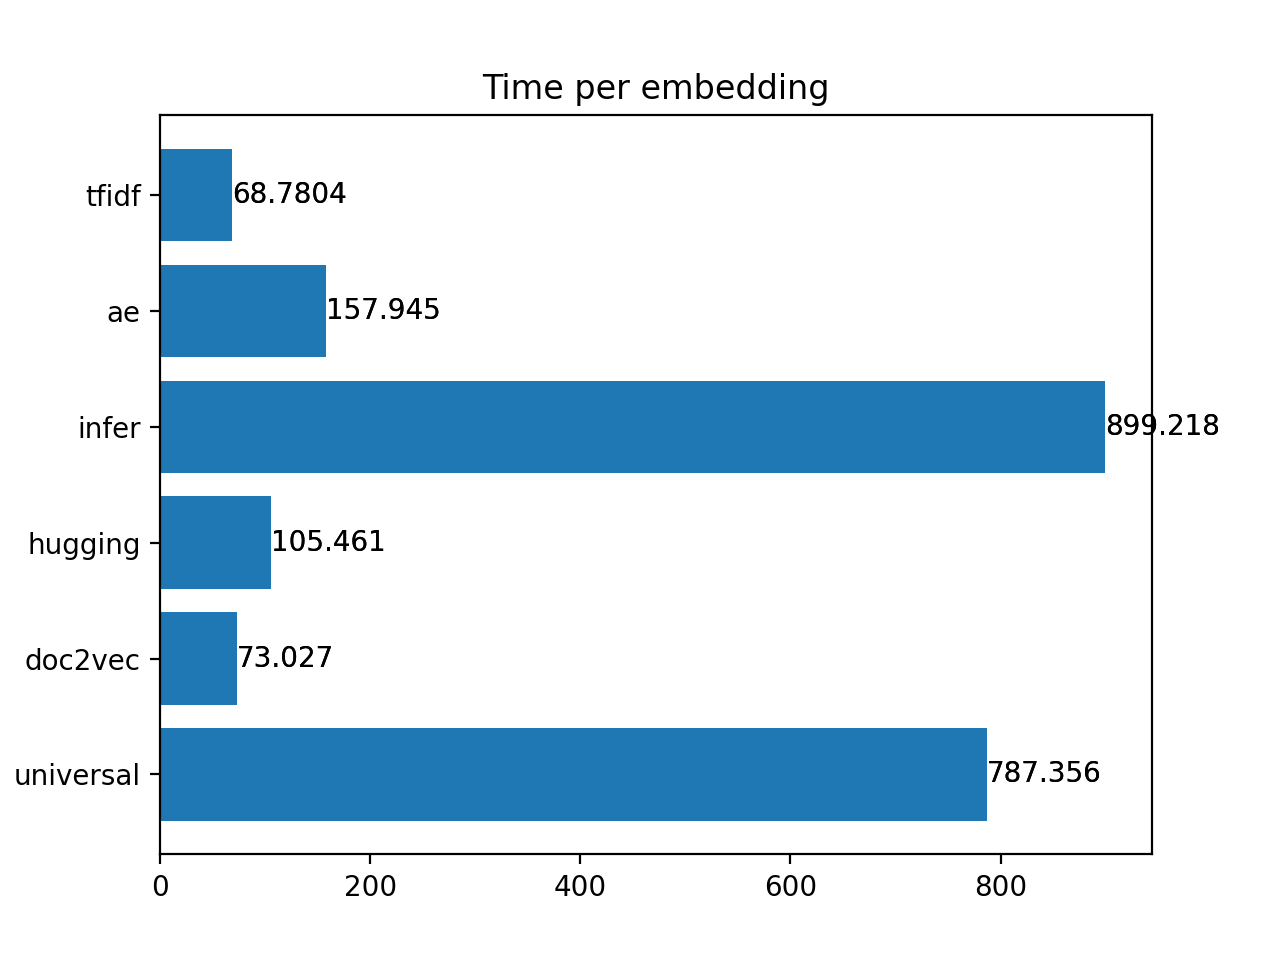
\includegraphics[width=5cm]{images/embeddings/infersent/time_per_doc_glove.png} }}%
    \qquad
    \subfloat[\centering Custom \ac{w2v} embeddings.]{{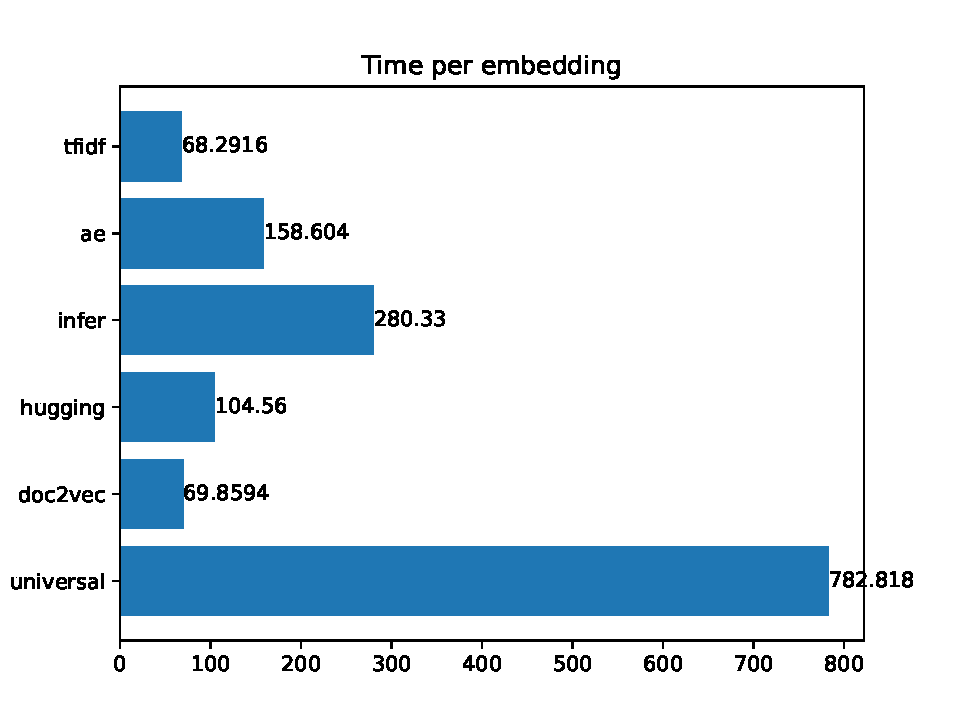
\includegraphics[width=5cm]{images/embeddings/infersent/time_per_doc_custom_emb.pdf} }}%
    \caption{Time (seconds) necessary to initialize the database, compute and insert 195 documents for specific embeddings.}%
    \label{fig:times_emb}%
\end{figure}


\section{Evaluation of \ac{use}}\label{sec:evaluation-use}

Since there are no parameters to customize the evaluation of the \ac{use} embeddings is limited.
Therefore, the \ac{use} embeddings are evaluated by comparing them to other embeddings.





\section{analysis/ comparison of models}\label{sec:evaluation-models}

% parameters
Similar to \citeauthor{glove2014}'s work, in this work, for many models used, any unspecified parameters are set to their default values, 
assuming that they are close to optimal
acknowledging that this simplification should be revised in a more thorough analysis.

% comparing models (qualitative)
difference query responses for different models?
any images which produce unusual results?

\section{Evaluation of the performance}\label{sec:evaluation-performance}

\subsection{Fahnder clustern}\label{subsec:evaluation-metric1}

\subsection{Fahnder bewerten Resultate (image matrix)}\label{subsec:evaluation-metric2}

\section{Evaluation of the usability}\label{sec:evaluation-usability}

\subsection{Metrics}\label{subsec:evaluation-metrics}